\documentclass[a4paper]{article}
\usepackage[T1]{fontenc}			% pacchetto per \chapter
\usepackage[italian]{babel}
\usepackage[italian]{isodate}  		% formato delle date in italiano
\usepackage{graphicx}				% gestione delle immagini
\usepackage{amsfonts}
\usepackage{booktabs}				% tabelle di qualità superiore
\usepackage{amsmath}				% pacchetto matematica
\usepackage{mathtools}				% per sottolineare sotto le equazioni
\usepackage{stmaryrd} 				% per '\llbracket' e '\rrbracket'
\usepackage{amsthm}					% teoremi migliorati
\usepackage{enumitem}				% gestione delle liste
\usepackage{pifont}					% pacchetto con elenchi carini
\usepackage{enumitem}				% pacchetto per elenchi con lettere dell'alfabeto
\usepackage{cancel}					% per cancellare delle espressioni matematiche
\usepackage{listings}				% implementa codice di programmazione


\usepackage[x11names]{xcolor}		% pacchetto colori RGB
% Link ipertestuali per l'indice
\usepackage{xcolor}
\usepackage[linkcolor=black, citecolor=blue, urlcolor=cyan]{hyperref}
\hypersetup{
	colorlinks=true
}

% Colour code style
\definecolor{codegreen}{rgb}{0,0.6,0}
\definecolor{codegray}{rgb}{0.5,0.5,0.5}
\definecolor{codepurple}{rgb}{0.58,0,0.82}
\definecolor{backcolour}{rgb}{0.95,0.95,0.92}

\lstdefinestyle{MATLAB}{
	backgroundcolor=\color{backcolour},   
	commentstyle=\color{codegreen},
	keywordstyle=\color{magenta},
	numberstyle=\tiny\color{codegray},
	stringstyle=\color{codepurple},
	basicstyle=\ttfamily\footnotesize,
	breakatwhitespace=false,         
	breaklines=true,                 
	captionpos=b,                    
	keepspaces=true,                 
	numbers=left,                    
	numbersep=5pt,
	showspaces=false,                
	showstringspaces=false,
	showtabs=false,                  
	tabsize=2
}
\lstset{style=MATLAB}

%\usepackage{showframe}				% visualizzazione bordi
%\usepackage{showkeys}				% visualizzazione etichetta

\newtheorem{theorem}{\textcolor{Red3}{\underline{Teorema}}}
\newtheorem{lemma}{Lemma}
\renewcommand{\qedsymbol}{QED}
\newcommand{\exec}[1]{\llbracket #1\:\rrbracket}
\newcommand{\dquotes}[1]{``#1''}
\newcommand{\longline}{\noindent\rule{\textwidth}{0.4pt}}

\begin{document}
	\author{Università degli Studi di Verona}
	\title{Simulazione di Elaborazione di segnali e immagini}
	\date{{\Large 22 Gennaio 2020}}
	\maketitle
	
	\section{Esercizio}
	
	Sia $g\left(t\right)$ un segnale di durata indefinita il cui spettro ideale analitico $G\left(\mu\right)$ è rappresentato in Figura 1.\newline
	
	\noindent
	(N.B.: NO repliche all'infinito, e con spettri NON nulli in $\left]-60,-30\right[, \left]-5,-5\right[, \left]30,60\right[$).
	
	\begin{figure}[!htp]
		\centering
		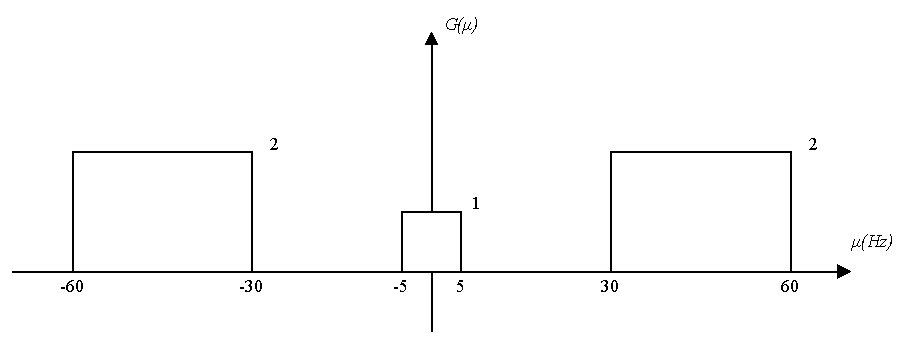
\includegraphics[width=\textwidth]{img/fig_1.pdf}
		\caption{Spettro ideale analitico $G\left(\mu\right)$.}
	\end{figure}
	
	\noindent
	Descrivere analiticamente in \underline{frequenza} e nel \underline{tempo} il segnale $g\left(t\right)$.\newpage
	
	\section{Esercizio}

	Descrivere inoltre:
	\begin{itemize}
		\item Analiticamente, nel \underline{tempo} e in \underline{frequenza}
		\item Graficamente, in \underline{frequenza}
	\end{itemize}
	Le elaborazioni a cui il segnale $g\left(t\right)$ (esercizio precedente) è sottoposto se ad esso vengono applicate le operazioni schematizzate dal sistema in Figura 2.\newline
	
	\noindent
	BONUS: Descrivere graficamente nel tempo $a\left(t\right), b\left(t\right), c\left(t\right)$.
	
	\begin{figure}[!htp]
		\centering
		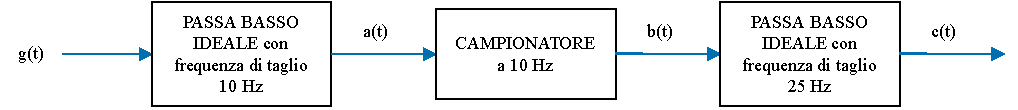
\includegraphics[width=\textwidth]{img/fig_2.pdf}
		\caption{Operazioni da applicare al segnale $g\left(t\right)$.}
	\end{figure}

	\section{Esercizio}
	
	Si risponda alle seguenti domande:
	\begin{enumerate}
		\item Descrivere cos'è l'istogramma di un’immagine, nella sua versione classica e probabilistica;
		
		\item Descrivere l'algoritmo che permette l'equalizzazione dell'istogramma;
		
		\item Descrivere che cos'è un filtro passa alto.
	\end{enumerate}
\end{document}